%%%%%%%%%%%%%%%%%%%%%%%%%%%%%%%%%%%%%%%%%%%%%%%%%%%%%%%%%%%%%%%%%%%%%%%%%%%%%%%
%
% REPORT  DESCRIPTION:
%   A concise description of the main concepts of the capstone.
%
% RESEARCH:
%   A list of research activities which led to this capstone.
%
% EXPERIMENTS:
%   A list of the experiments performed which supported the research.
%
%%%%%%%%%%%%%%%%%%%%%%%%%%%%%%%%%%%%%%%%%%%%%%%%%%%%%%%%%%%%%%%%%%%%%%%%%%%%%%%
\documentclass[12pt,american]{report}
\usepackage{rit-cs-capstone}
%%%%%%%%%%%%%%%%%%%%%%%%%%%%%%%%%%%%%%%%%%%%%%%%%%%%%%%%%%%%%%%%%%%%%%%%%%%%%%%
%   The following packages are all optional and depend on the specifics of what
% is contained in the capstone.  There is no harm in leaving them in.
%%%%%%%%%%%%%%%%%%%%%%%%%%%%%%%%%%%%%%%%%%%%%%%%%%%%%%%%%%%%%%%%%%%%%%%%%%%%%%%
\usepackage{subfigure}
\usepackage[refpages]{gloss}
\usepackage{babel}
\usepackage{times}
\usepackage{graphicx}
\usepackage{amssymb}
\usepackage{lscape}
\usepackage{verbatim}
\usepackage{enumerate}
\usepackage{afterpage}
\usepackage{booktabs}
%%%%%%%%%%%%%%%%%%%%%%%%%%%%%%%%%%%%%%%%%%%%%%%%%%%%%%%%%%%%%%%%%%%%%%%%%%%%%%%
%   Mark the document as 'draft' with a date. Be sure to comment this out for
% the final version.
\usepackage{watermark}
\watermark{\hspace{-0.3in} \textbf{DRAFT} \hspace{2.0in} \textbf{\today}}
%%%%%%%%%%%%%%%%%%%%%%%%%%%%%%%%%%%%%%%%%%%%%%%%%%%%%%%%%%%%%%%%%%%%%%%%%%%%%%%

\makegloss

\begin{document}
%%%%%%%%%%%%%%%%%%%%%%%%%%%%%%%%%%%%%%%%%%%%%%%%%%%%%%%%%%%%%%%%%%%%%%%%%%%%%%%
% Title page
% The \title{} can contain line breaks as appropriate...
\title{\vspace{-0.20in}Icosatree Data Partitioning of\\
Massive Geospatial Point Clouds\\
with User-Selectable Entities and\\
Surface Modeling}
% The \titleline{} must have no line breaks in it.
\titleline{Icosatree Data Partitioning of Massive Geospatial Point Clouds with
User-Selectable Entities and Surface Modeling}
% This is not a project but a thesis
\MSprojectfalse
% This date is really not used (unless \grantdate{}{} is blank)
\date{Month Year}
%%%%%%%%%%%%%%%%%%%%%%%%%%%%%%%%%%%%%%%%%%%%%%%%%%%%%%%%%%%%%%%%%%%%%%%%%%%%%%%

%%%%%%%%%%%%%%%%%%%%%%%%%%%%%%%%%%%%%%%%%%%%%%%%%%%%%%%%%%%%%%%%%%%%%%%%%%%%%%%
% Author information page
% The \author{} should be exactly the same as your diploma
\author{Stephen Ranger}
%%%%%%%%%%%%%%%%%%%%%%%%%%%%%%%%%%%%%%%%%%%%%%%%%%%%%%%%%%%%%%%%%%%%%%%%%%%%%%%

%%%%%%%%%%%%%%%%%%%%%%%%%%%%%%%%%%%%%%%%%%%%%%%%%%%%%%%%%%%%%%%%%%%%%%%%%%%%%%%
% The following information is for the signature page.
% Note that the definition for principal adviser uses two fields.
% This was needed so that the adviser's name could be placed on the
% abstract page without his/her title.
\committeechair{Dr. Reynold Bailey}{Associate Professor\\Associate Undergraduate Program Coordinator}
\reader{Dr. Joe Geigel\\Professor}
\observer{Dr. Zack Butler\\Associate Professor\\Associate Graduate Coordinator}
%%%%%%%%%%%%%%%%%%%%%%%%%%%%%%%%%%%%%%%%%%%%%%%%%%%%%%%%%%%%%%%%%%%%%%%%%%%%%%%

%%%%%%%%%%%%%%%%%%%%%%%%%%%%%%%%%%%%%%%%%%%%%%%%%%%%%%%%%%%%%%%%%%%%%%%%%%%%%%%
% This is the expected date that the committee will sign your Capstone.
\grantdate{December}{2016}
%%%%%%%%%%%%%%%%%%%%%%%%%%%%%%%%%%%%%%%%%%%%%%%%%%%%%%%%%%%%%%%%%%%%%%%%%%%%%%%

%%%%%%%%%%%%%%%%%%%%%%%%%%%%%%%%%%%%%%%%%%%%%%%%%%%%%%%%%%%%%%%%%%%%%%%%%%%%%%%
% If you want to copyright your capstone remove the line below.
\copyrightfalse% True by default
% The year of the copyright; usually same as the date the committee will
% sign the \item{} . This won't be printed if \copyrightfalse
\copyrightyear{2016}
%%%%%%%%%%%%%%%%%%%%%%%%%%%%%%%%%%%%%%%%%%%%%%%%%%%%%%%%%%%%%%%%%%%%%%%%%%%%%%%

%%%%%%%%%%%%%%%%%%%%%%%%%%%%%%%%%%%%%%%%%%%%%%%%%%%%%%%%%%%%%%%%%%%%%%%%%%%%%%%
% This causes all front matter to be set.
\beforepreface%
%%%%%%%%%%%%%%%%%%%%%%%%%%%%%%%%%%%%%%%%%%%%%%%%%%%%%%%%%%%%%%%%%%%%%%%%%%%%%%%

%%%%%%%%%%%%%%%%%%%%%%%%%%%%%%%%%%%%%%%%%%%%%%%%%%%%%%%%%%%%%%%%%%%%%%%%%%%%%%%
% The dedication - if you choose to include one.
% It should be vertically centered in the page. Since the style format doesn't 
% do it for you automatically, you can use the following technique.
\prefacesection{Dedication}
\vfill
\begin{center}
I'd like to dedicate this to my wife; she's been supportive of
me throughout all my procrastination and frustration.
\end{center}
\vfill
%%%%%%%%%%%%%%%%%%%%%%%%%%%%%%%%%%%%%%%%%%%%%%%%%%%%%%%%%%%%%%%%%%%%%%%%%%%%%%%

%%%%%%%%%%%%%%%%%%%%%%%%%%%%%%%%%%%%%%%%%%%%%%%%%%%%%%%%%%%%%%%%%%%%%%%%%%%%%%%
% The acknowledgements page - if you choose to include one. 
% As in the dedication, it should be centered vertically in the page.
%
%\prefacesection{Acknowledgments}
%\vfill
%\begin{center}
%\indent I am grateful for ...
%\end{center}
%\vfill
%%%%%%%%%%%%%%%%%%%%%%%%%%%%%%%%%%%%%%%%%%%%%%%%%%%%%%%%%%%%%%%%%%%%%%%%%%%%%%%

%%%%%%%%%%%%%%%%%%%%%%%%%%%%%%%%%%%%%%%%%%%%%%%%%%%%%%%%%%%%%%%%%%%%%%%%%%%%%%%
%%  Collection of useful abbreviations.
\newcommand{\etc} {\emph{etc.\/}}
\newcommand{\etal}{\emph{et~al.\/}}
\newcommand{\eg}  {\emph{e.g.\/}}
\newcommand{\ie}  {\emph{i.e.\/}}
%%%%%%%%%%%%%%%%%%%%%%%%%%%%%%%%%%%%%%%%%%%%%%%%%%%%%%%%%%%%%%%%%%%%%%%%%%%%%%%


%%%%%%%%%%%%%%%%%%%%%%%%%%%%%%%%%%%%%%%%%%%%%%%%%%%%%%%%%%%%%%%%%%%%%%%%%%%%%%%
% Abstract
\begin{abstractpage}
Massive point cloud data sets are currently being created and studied in
academia, the private sector, and the military. Many previous attempts at
rendering point clouds have allowed the user to visualize the data in a
three-dimensional way but did not allow them to interact with the data and would
require all data to be in memory at runtime. Recently, a few systems have
cropped up that deal with real-time rendering of massive point clouds with
on-the-fly level of detail modification that handles out-of-core processing but
these systems have their own limitations. With the size and scale of massive
point cloud data coming from LiDAR (Light Detection and Ranging) systems, being
able to visualize the data as well as interact and transform the data is needed.

Previous work in out-of-core rendering
\cite{3_wenzel2014out,4_goswami_zhang_pajarola_gobbetti_2010,5_richter_2010}
showed that using Octrees and K-D Trees can increase the availability of data as
well as allow a user to visualize the information in a much more useful manner.
However, viewing the data isn't enough; applying work in context-aware selection
\cite{2_yu:hal-01178051} and surface creation \cite{1_VAST:VAST11:105-112} the
visualization system would greatly benefit in usability and functionality.
\end{abstractpage}

%%%%%%%%%%%%%%%%%%%%%%%%%%%%%%%%%%%%%%%%%%%%%%%%%%%%%%%%%%%%%%%%%%%%%%%%%%%%%%%

%%%%%%%%%%%%%%%%%%%%%%%%%%%%%%%%%%%%%%%%%%%%%%%%%%%%%%%%%%%%%%%%%%%%%%%%%%%%%%%
% Uncomment the line below if you don't want a list of tables to be printed.
% \tablespagefalse

% Uncomment the line below if you don't want a list of figures to be printed.
% \figurespagefalse

% \afterpreface generates the table of contents, list of tables (optional),
% and list of figures (optional).
\afterpreface%
%%%%%%%%%%%%%%%%%%%%%%%%%%%%%%%%%%%%%%%%%%%%%%%%%%%%%%%%%%%%%%%%%%%%%%%%%%%%%%%

%We don't need a glossary so comment it out.
%\printgloss{Glossary}

%%%%%%%%%%%%%%%%%%%%%%%%%%%%%%%%%%%%%%%%%%%%%%%%%%%%%%%%%%%%%%%%%%%%%%%%%%%%%%%
% This is where the main body of the capstone report starts
\body%

\chapter{Introduction}

% % Obviously you need to delete these lines when you have written up your text

Massive point cloud datasets are becoming more prevalent as technology becomes
cheaper and storage and rendering power grow leaps and bounds. This thesis
attempts to demonstrate a novel partitioning structure called an Icosatree as
well as a three dimensional triangular coordinate used for positioning values
inside the data structure. This icosahedron-based three dimensional data
partitioning structure was developed in order to address a few failings seem
with common data structures used for these types of datasets, such as the
Octree. The algorithm itself is explained further in Chapter 3.

First, the Octree being axis-aligned is poorly suited to the projected surface
the data is displayed in. This causes the cells in the tree to look asymmetrical
and as each subsequent layer of the tree is displayed the asymmetrical nature of
the visualization becomes more apparent. With the Icosatree, each cell is more
closely aligned with the projected geospatial surface and each cell appears as a
triangular area to the user. In the final visualization, the cells are added as
they are accessed from the data source (local file system or HTTP requests) and
as they are added to the rendering element it does indeed look much more
uniform.

Second, with the Icosatree being much closer to the projected geospatial surface
the hope is that less cells would be required in the output dataset and would
more efficiently fill our rendering data structure. This has been seen to be the
case, however, with limited resources on commodity graphics hardware a sweet
spot between performance and data utilization was more difficult to determine
automatically by the system and needs improvement. This will be covered in more
depth in the future work section at the end of this paper.

The Icosatree also uses a new triangular coordinate system in order to position
points into the Icosatree cells, or Icosatet. The Icosatet is a triangular prism
that is used as the basic sub-structure in the Icosatree. The initial Icosatree
is split into twenty Icosatets and each subsequent level in the tree splits each
Icosatet into eight smaller Icosatets. The triangular coordinates used allow the
points in each level of the Icosatree to be as uniformly distributed as
possible. This new coordinate system is explained in Chapter 4.

The resulting visualization was then used to test a hybrid user-definable
triangulation algorithm loosely based on the work found in two separate papers
[1,2]. The general idea behind this augmented algorithm is that the user selects
a region of the screen and any points within that area are selected. This set of
points will then be pruned using a combination of nearest neighbor density
values, eigenvector comparisons between the entire selection and nearest
neighbors, and altitude thresholds which are all definable by the user. Next,
the set can be limited further by removing any points hidden by others based on
a ray casting and occlusion test. Finally, the resulting set of points are fed
into a Delaunay triangulation algorithm in order to create a triangle mesh.
\chapter{Background}

The basis for this continued work stems from multi-dimensional data structures
and how they are leveraged in a geospatial environment. These data structures,
the Quadtree, Octree, and K-D Tree, are used to partition a (usually) Cartesian
coordinate system into a tree structure.

\section{Quadtree}

The Quadtree separates a two-dimensional coordinate system into a tree structure
where each node in the tree is split along the center of both axes within its
axis-aligned bounding volume creating four child nodes. This allows for much
more efficient searching than a simple data structure like an array or list
would. Below, \ref{fig:quadtree} shows a set of points in a two-dimensional
Cartesian coordinate system stored in a Quadtree where each node that has only a
single point remaining does not split again; thus saving computational time and
storage space. The Quadtree structure is used in geospatial visualizations as it
aligns to the longitude and latitude coordinate system, however, the disconnect
along the 180-degree meridian and the difficult-to-handle north and south border
meeting at a single point cause more issues.

\begin{figure}[htb]
\begin{center}
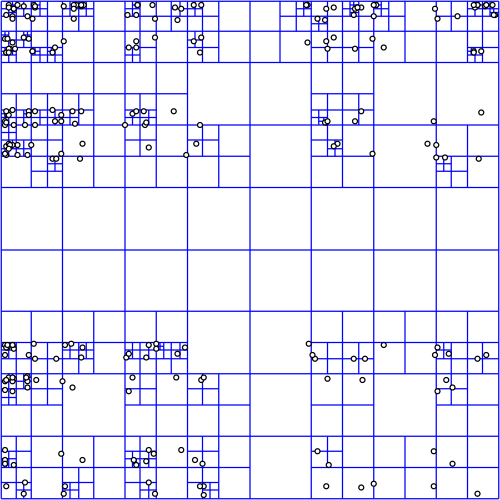
\includegraphics[width=.5\linewidth]{images/Point_quadtree.png}
\end{center}
\caption{Quadtree Structure {\cite{10_eppstein_2005}}}
\label{fig:quadtree}
\end{figure}

\section{Octree}

The Octree structure is identical to the Quadtree structure except that it is
applied to a three-dimensional coordinate system. Each node is split into
potentially eight child nodes but it still uses a uniform split location by
bisecting the span along each axis of its axis-aligned bounding volume. The
Octree is used quite often in Computer Graphics as it fits well to an XYZ
Cartesian coordinate system and allows culling, bounds intersection, and mouse
picking for many objects quickly and efficiently. However, in a geospatial
visualization, this structure does not align well to an elliptical surface such
as the Earth. Below, \ref{fig:octree} is an image of an Octree in 3D as well as the
flattened version of the tree.

\begin{figure}[htb]
\begin{center}
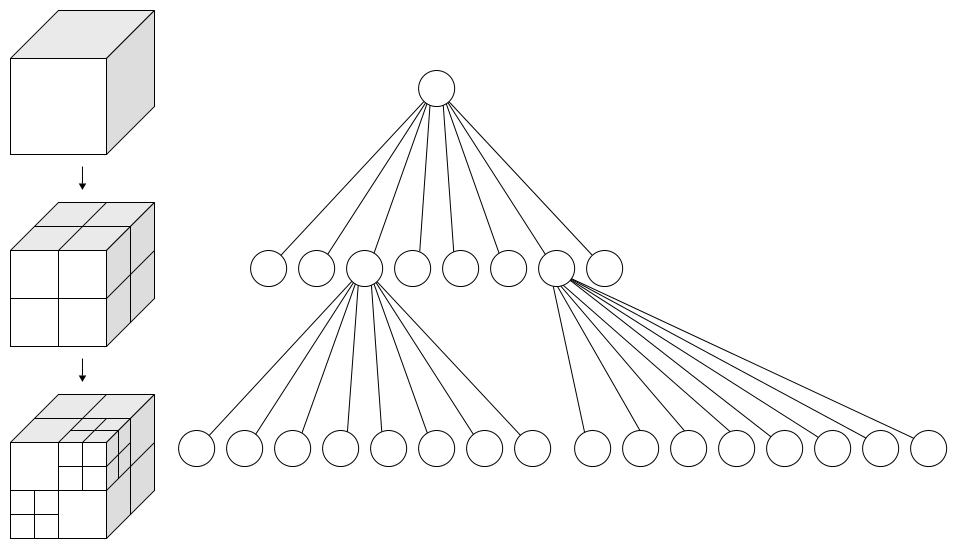
\includegraphics[width=.9\linewidth]{images/Octree_flat.png}
\end{center}
\caption{Octree Structure and Flattened Tree \cite{11_octree2.png}}
\label{fig:octree}
\end{figure}

\section{k-d tree}

The K-D Tree is a specialized binary tree that allows for more control over how
the tree is structured as well as lending itself to being more uniform and
balanced than previously mentioned tree data structures. The K-D Tree, at each
level, chooses a single axis to split along. The axis chosen is defined by a set
of criteria such as which axis has the longest span between its min and max
values. Then, the split location is also defined by a set of criteria such as
splitting each side into containing a uniform number of points. The actual split
location, unlike the Quadtree and Octree, is a single point that acts as the
node in the tree at that depth. This continues until each node has a single
point or until some threshold is reached based on tree depth or point count. The
K-D Tree is a binary tree but can be used with any dimensionality which allows
it to be applied to a two-dimensional longitude-latitude coordinate system as
with the Quadtree and an XYZ Cartesian coordinate system like the Octree. It has
many of the same drawbacks when it comes to applying it to a geospatial
coordinate system. However, one upside is that it can be built in such a way
that each node has a relatively uniform number of points which can increase
storage efficiency and render times by allowing the storage of nodes in chunks
without wasting padded space but with the drawback that level-of-detail
algorithms make the scene seem non-uniform as each node is rendered and the node
dimensions are not consistent. Below, \ref{fig:kdtree2d} shows a two-dimensional K-D Tree
partitioning algorithm with red and blue lines as alternating split locations.
\ref{fig:kdtreelayers} shows the flattened tree structure for part of the previous figure and
which axis was used at each level.

\begin{figure}[htb]
\begin{center}
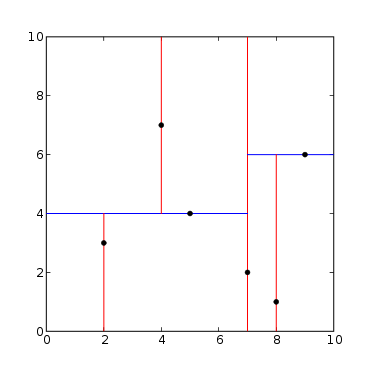
\includegraphics[width=.5\linewidth]{images/kdtree_2d.png}
\end{center}
\caption{Two-Dimensional K-D Tree Structure \cite{12_kdtree_2d.svg}}
\label{fig:kdtree2d}
\end{figure}

\begin{figure}[htb]
\begin{center}
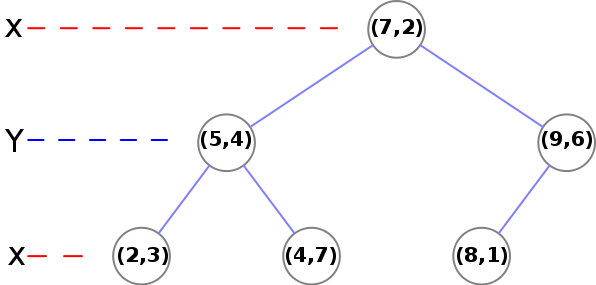
\includegraphics[width=.5\linewidth]{images/kdtree_layers.png}
\end{center}
\caption{K-D Tree Partitioning Example \cite{13_tree_0001.svg}}
\label{fig:kdtreelayers}
\end{figure}

Previously, Quadtree, Octree \cite{3_wenzel2014out} and K-D Tree partitioning
systems have been applied to a Cartesian system in order to add on-demand
searching for view-dependent slices of data. However, once the data set is
converted into a geospatial positioning system, either the Cartesian coordinates
are now not surface aligned, or issues arise along the partitioning system
boundaries where values are not continuous (such as with latitude 90 != latitude
-90 but longitude 180 == longitude -180). Using a Cartesian projection from
geospatial coordinates solves this issue but adds complexity when deciding what
to render as it is no longer surface aligned. This paper looks into applying a
surface-aligned data structure to a global data set such as a tetrahedral mesh.
By using this structure to search for nodes within the view frustum the
visualization system will be able to render progressively deeper nodes as the
visualization's viewpoint moves closer or further away from the target and as
the level of detail increases and will then pull these nodes from an on-demand
point server or local file system cache.

Also, in recent work, real-time rendering of depth culling and surface
representation \cite{1_VAST:VAST11:105-112} has been used to hide unseen data
points as well as to fill surface information in on a massive unstructured point
cloud. This paper proposes to use this information and apply it to a sparse
context-aware selection algorithm \cite{2_yu:hal-01178051} in order to adapt it
to a more uniformly dense data set. This on-the-fly surface creation can be used
to augment the context-aware selection algorithm in order to give it another
avenue for object separation qwithin a uniformly-dense data set.

\chapter{Design}

%% Obviously you need to delete these lines when you have written up your text
\begin{itemize}
\item{} How you designed your solution
\item{} Rationale for decisions
\item{} Compare and contrast design with other approaches (related work) 
\end{itemize}
\chapter{Implementation}

The system designed for this research contains four major pieces: A Partitioning
application, A Visualization tool, The Rendering Component, and the Selection
Algorithm. Below is a detailed explanation of their implementation and theory.

\section{Partitioning Application}

The partitioning application is a standalone command line application that reads
from a number of binary point data files. It creates the different partitioning
systems needed to evaluate the algorithm implementations and stores them in a
custom binary format for ease of access at runtime. The files have been designed
so that they can be accessed via the local file system or through a web server.

The data structure has been partitioned such that each level in the tree
structure, for both the Octree and Icosatree, contains points which are left in
each node. The nodes are split into a sub-cell grid structure so all nodes at a
specific depth are uniformly dense in order for the level of detail algorithm to
only have to deal with screen area and not point densities within the
visualization tool when determining how deep to traverse. The data also contains
information defining the number of points in the node, the number of child
nodes, and the layout of the binary data (at the root, only).

The structure of the Octree and Icosatree file systems are fairly
straightforward. Each is defined by a file tree originating at a given root
directory. Then in each directory, including the root, a point data file exists
along with an ASCII text file containing a list of the existing child nodes at
that location. The root directory also contains a CSV file defining the binary
layout of the point data which contains information about attributes: name,
offset, data type, size in bytes, min, max, mean, and variance.

The Octree and Icosatree structures are identical except for the fact that each
Octree cell contains, at most, eight child cells. The Icosatree root node can
contain up to twenty child cells and each cell after that can contain at most
eight. The Octree structure is split along the XYZ axes as in Figure 2. However,
the Icosatree is split into twenty triangular prism cells at the root as in
Figure 5. Below that, each cell is split into eight additional triangular prisms
as seen in Figure 6 and Figure 7.

\begin{figure}[htp]
\begin{center}
  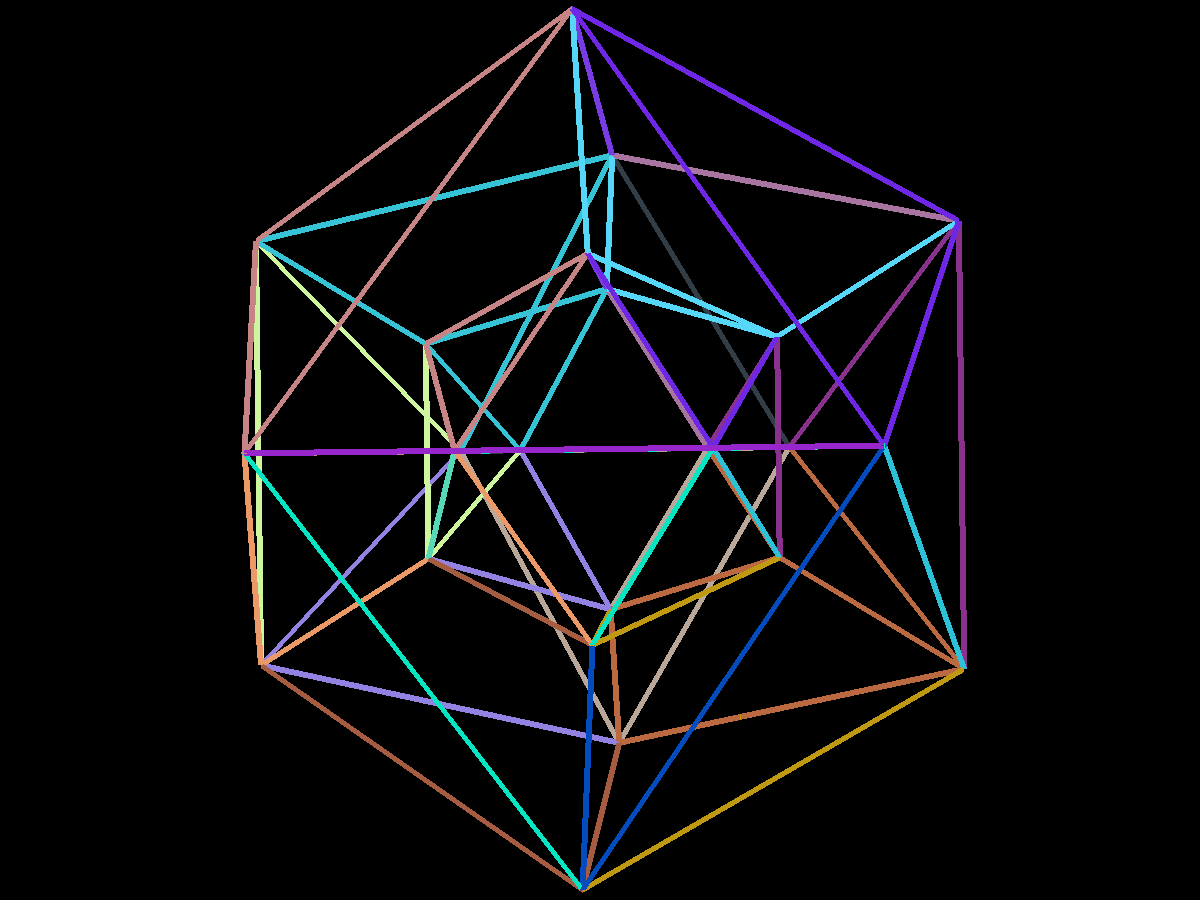
\includegraphics[width=.75\linewidth]{images/trianglePrismBounds.png}
  \caption{Icosatree Wireframe}
  \label{fig:tpv}
\end{center}
\end{figure}

\begin{figure}[htp]
\begin{center}
  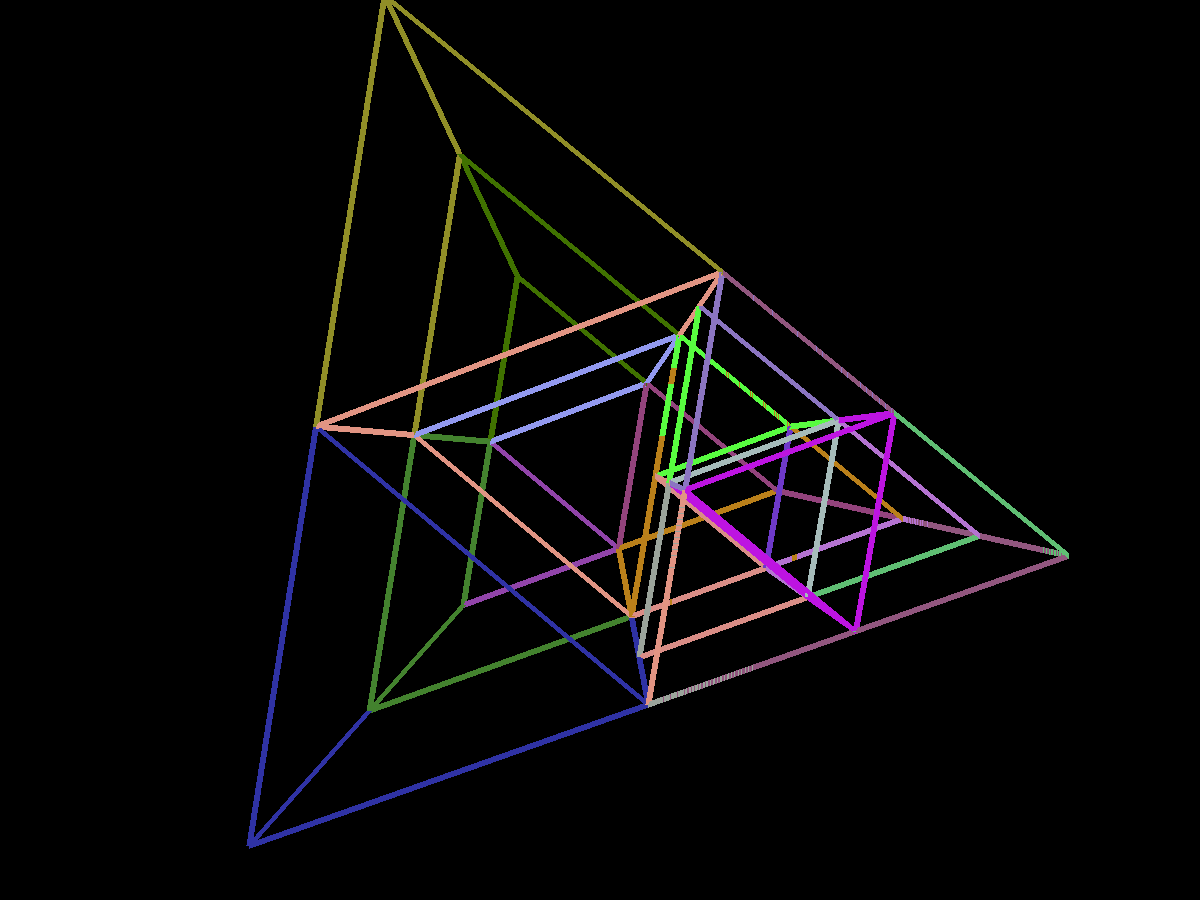
\includegraphics[width=.75\linewidth]{images/trianglePrismBoundsSplit.png}
  \caption{Triangle Prism Partitioning}
  \label{fig:tpvSplit}
\end{center}
\end{figure}

\begin{figure}[htp]
\begin{center}
  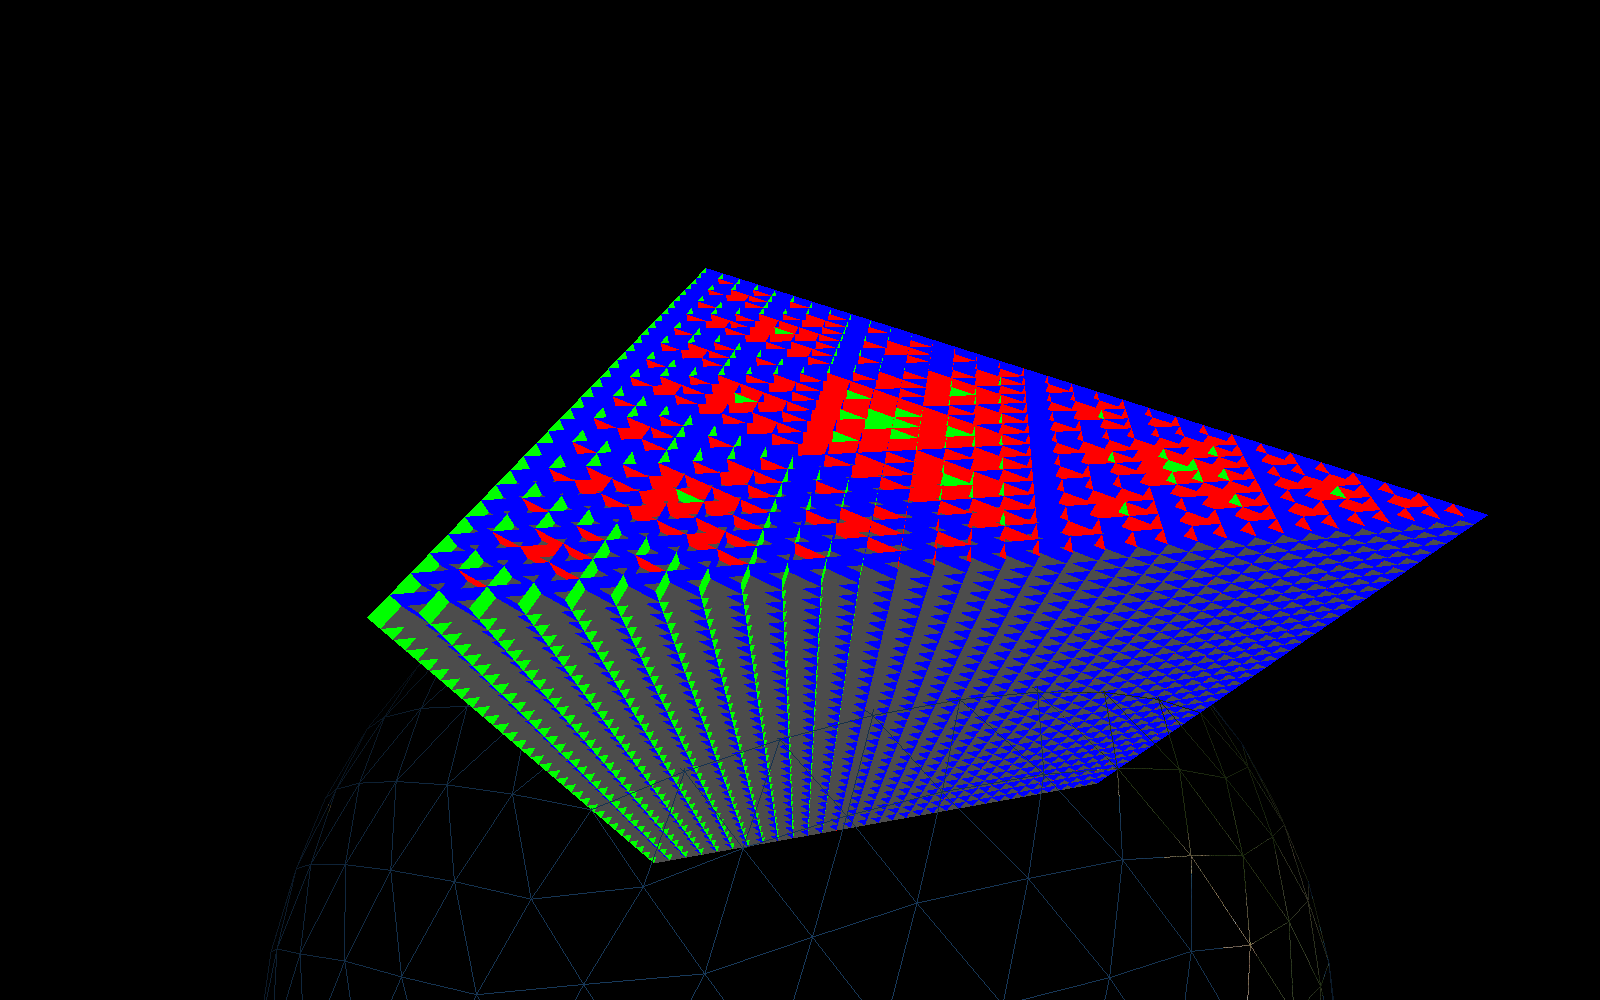
\includegraphics[width=.9\linewidth]{images/treeStructure_depth5.png}
  \caption{Icosatree Cells - Depth 5}
  \label{fig:icosatreeCells}
\end{center}
\end{figure}

Each cell is also split into sub-cells; this allows the tree creation to
guarantee uniform density of point data at any specific level of the tree which
greatly simplifies level of detail calculations in the renderer. As the tree
structure is built, a point is inserted into the root node. The sub-cell is
computed and if no point was previously added there, the current point is
stored. If a point was previously stored at that sub-cell index, the point
closest to its centroid is left there and the remaining point is sent to one of
the cells' child cells. This continues until all points have been added to the
tree. Once that is complete, the command line tool writes the tree structure as
a set of directories and binary or ASCII files. A subset of this file structure
can be seen in \ref{fig:fileStructure}. The DAT file contains the binary point data and the
text file contains the child cell index values which contain point data of their
own. These child cells also have a sub-directory within that nodes’ directory
which continues to the leaves of the tree.

\begin{figure}[htp]
\begin{center}
  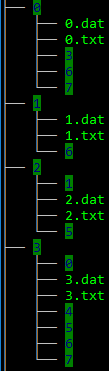
\includegraphics[height=3.0in]{images/filestructure.png}
  \caption{Tree File Structure}
  \label{fig:fileStructure}
\end{center}
\end{figure}

\section{Visualization Tool}

The visualization tool consists of a Java/OpenGL rendering system based off the
Java OpenGL Library (JOGL) and a rendering toolkit the author has developed.
Simple geospatial navigation and terrestrial terrain have been added as they aid
the user when interacting and visualizing this form of data. The visualization
renders a simple WGS84 projected globe, a spherical orbit navigator, the point
cloud renderer which supports the different data structures implemented by the
partitioning application, and the selection algorithm used by the user which
allows them to select objects, as the points that comprise them, from the scene
using a screen-space lasso tool.

The visualization tool renders each item in the scene as its own scene element.
The camera navigation is based on a geospatial anchor point and an
azimuth/elevation/distance offset from the anchor. A local origin will offset
the scene component's local coordinate system for floating point precision
reasons and each scene element will update its own position based on this local
origin.

There was also the need for a renderable Earth scene element \ref{fig:earth}.
This was developed by creating a GeodesicCoordinate to base the geometry from. The first level of
detail consists of a number of rectangular sections each thirty degrees on a
side. Then, as the camera moves closer to the surface, each portion splits into
smaller sections \ref{fig:earthWire}. In order to display accurate elevation
data, support for Digital Elevation Model data was added and used as a lookup
dataset for elevation values at each vertex \ref{fig:earthDEM}. Initially, a
single high resolution texture was used for the imagery but even an 8k image did
not add enough fidelity as the user zoomed close enough into the terrain so
support was also added for the Slippy Map Tile URL protocol; specifically,
OpenStreetMap and Stamen Terrain imagery \ref{fig:earthTiles}. The Digital
Elevation Model data is downloadable manually and is indexed the first time the
Visualization application is run whereas the imagery is accessed via HTTP
requests as it is needed.

\begin{figure}[htp]
\begin{center}
  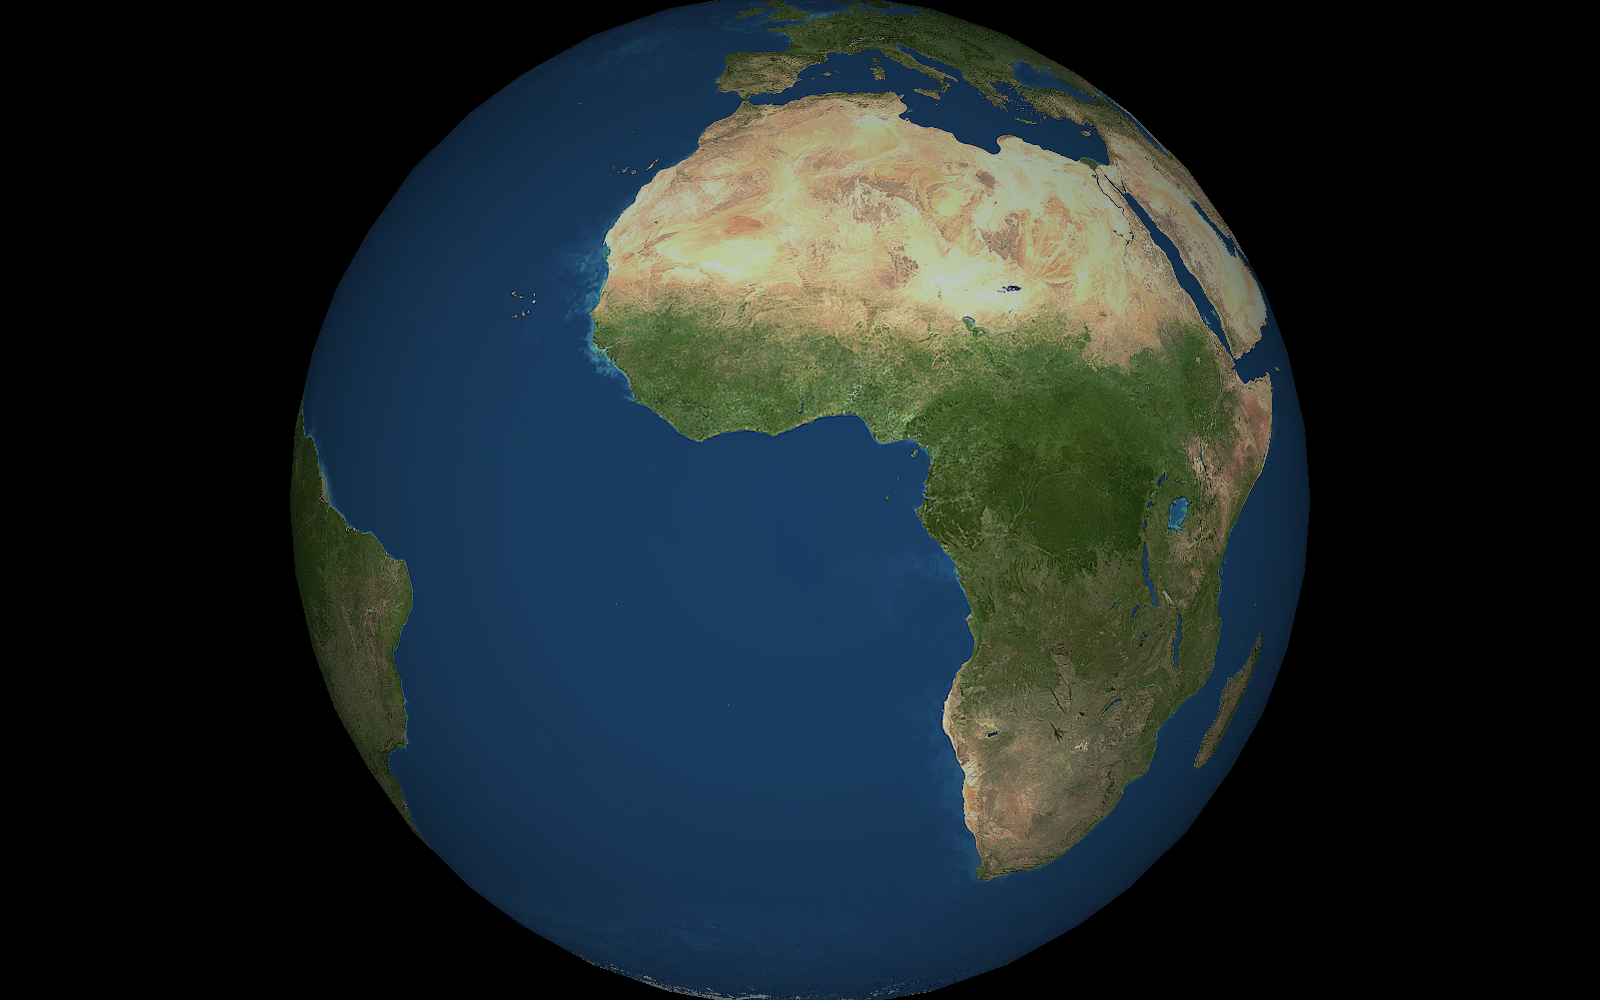
\includegraphics[width=.75\linewidth]{images/earth.png}
  \caption{Earth}
  \label{fig:earth}
\end{center}
\end{figure}

\begin{figure}[htp]
\begin{center}
  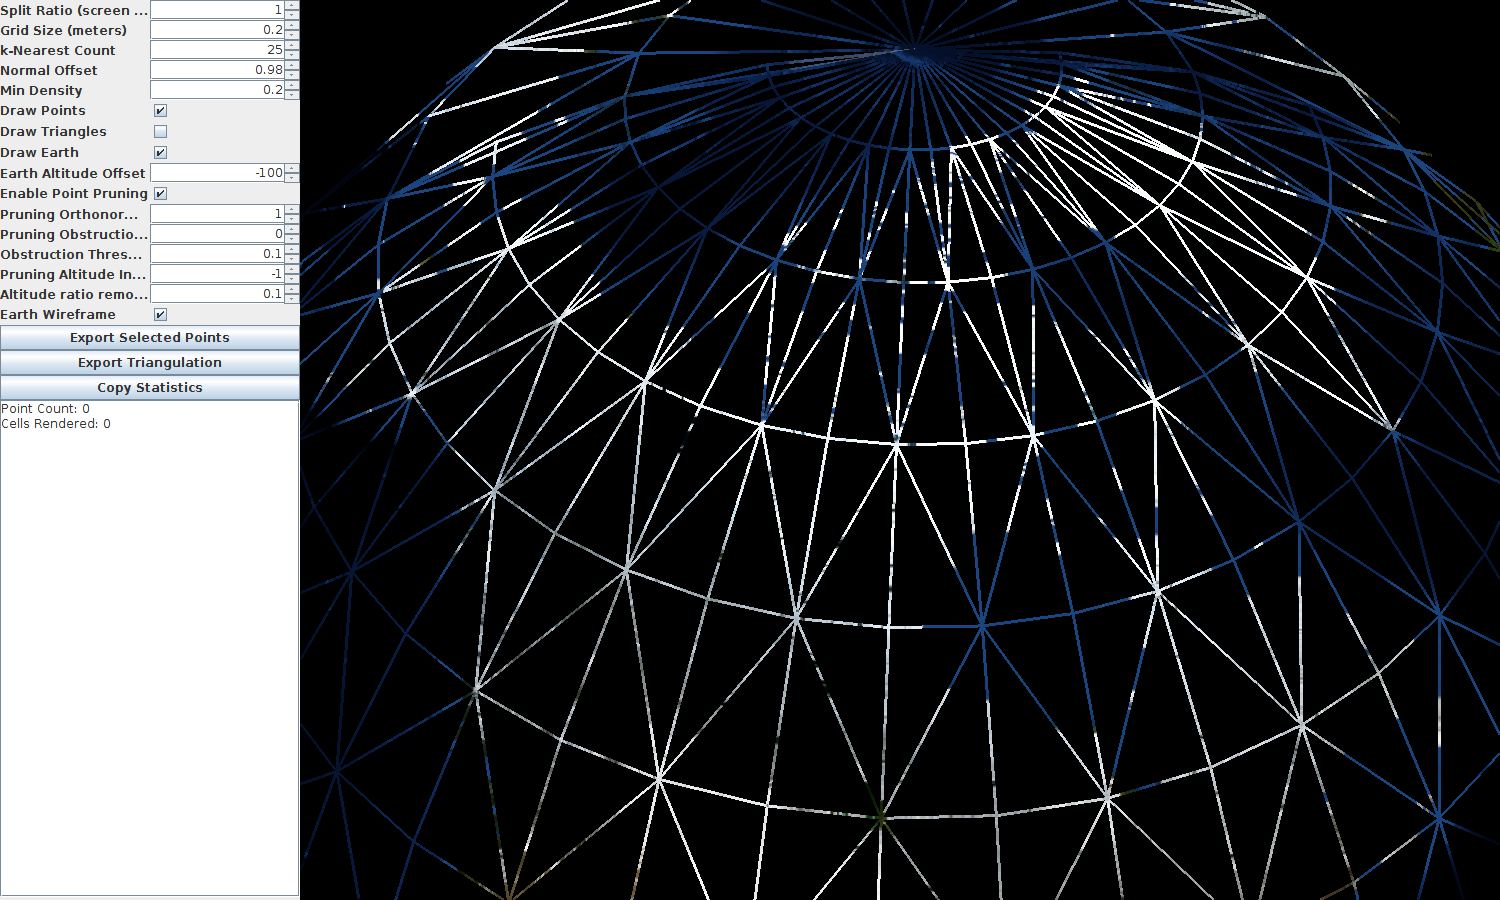
\includegraphics[width=.75\linewidth]{images/earthlod.png}
  \caption{Earth Wireframe}
  \label{fig:earthWire}
\end{center}
\end{figure}

\begin{figure}[htp]
\begin{center}
  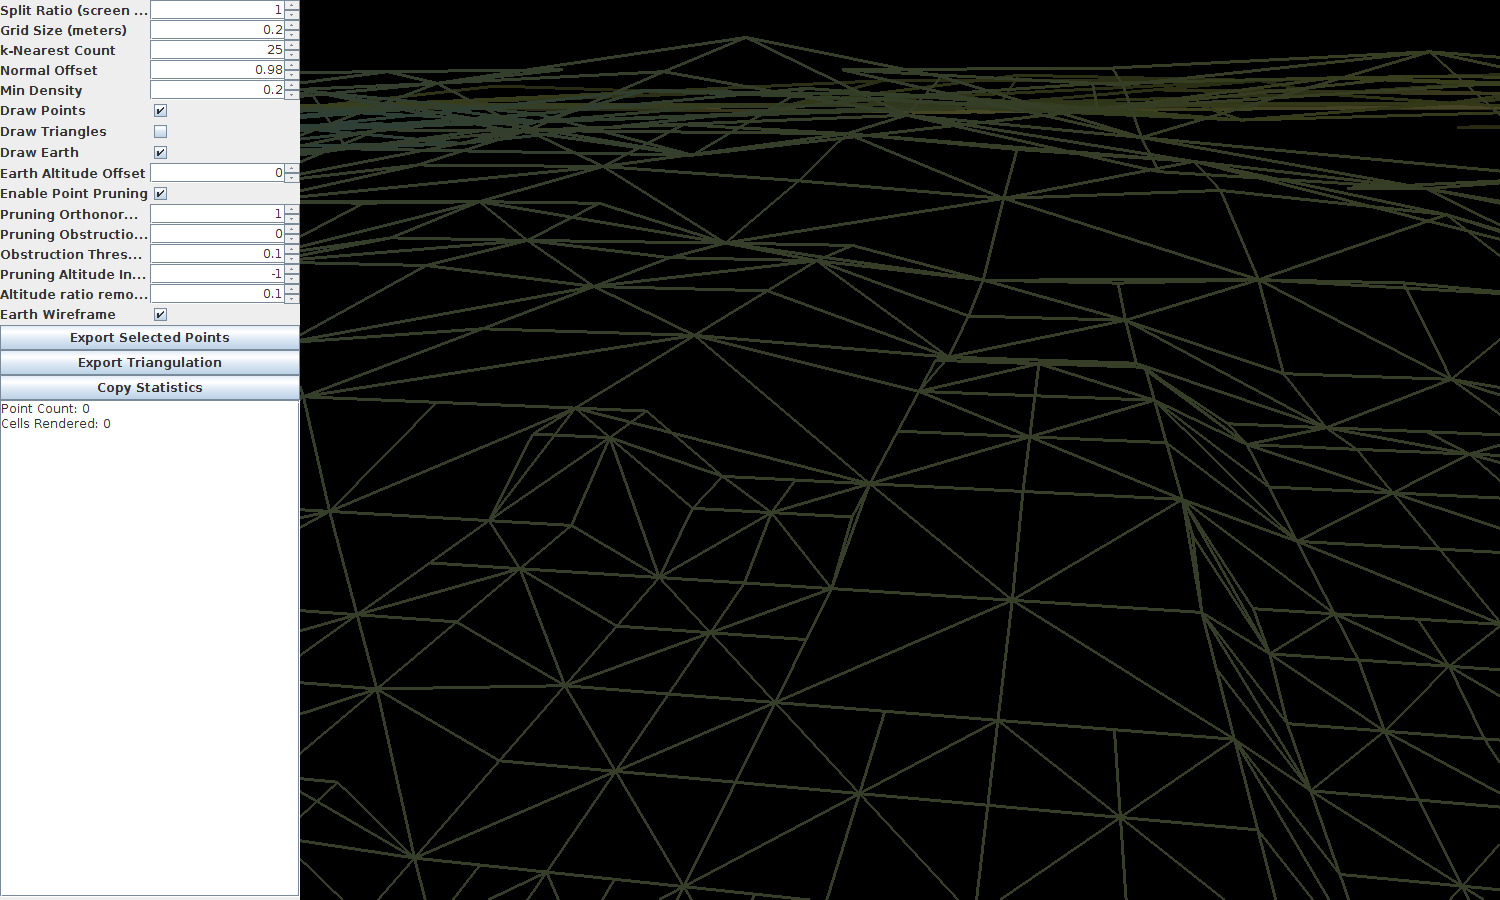
\includegraphics[width=.75\linewidth]{images/earthElevation.png}
  \caption{Earth Elevation}
  \label{fig:earthDEM}
\end{center}
\end{figure}

\begin{figure}[htp]
\begin{center}
  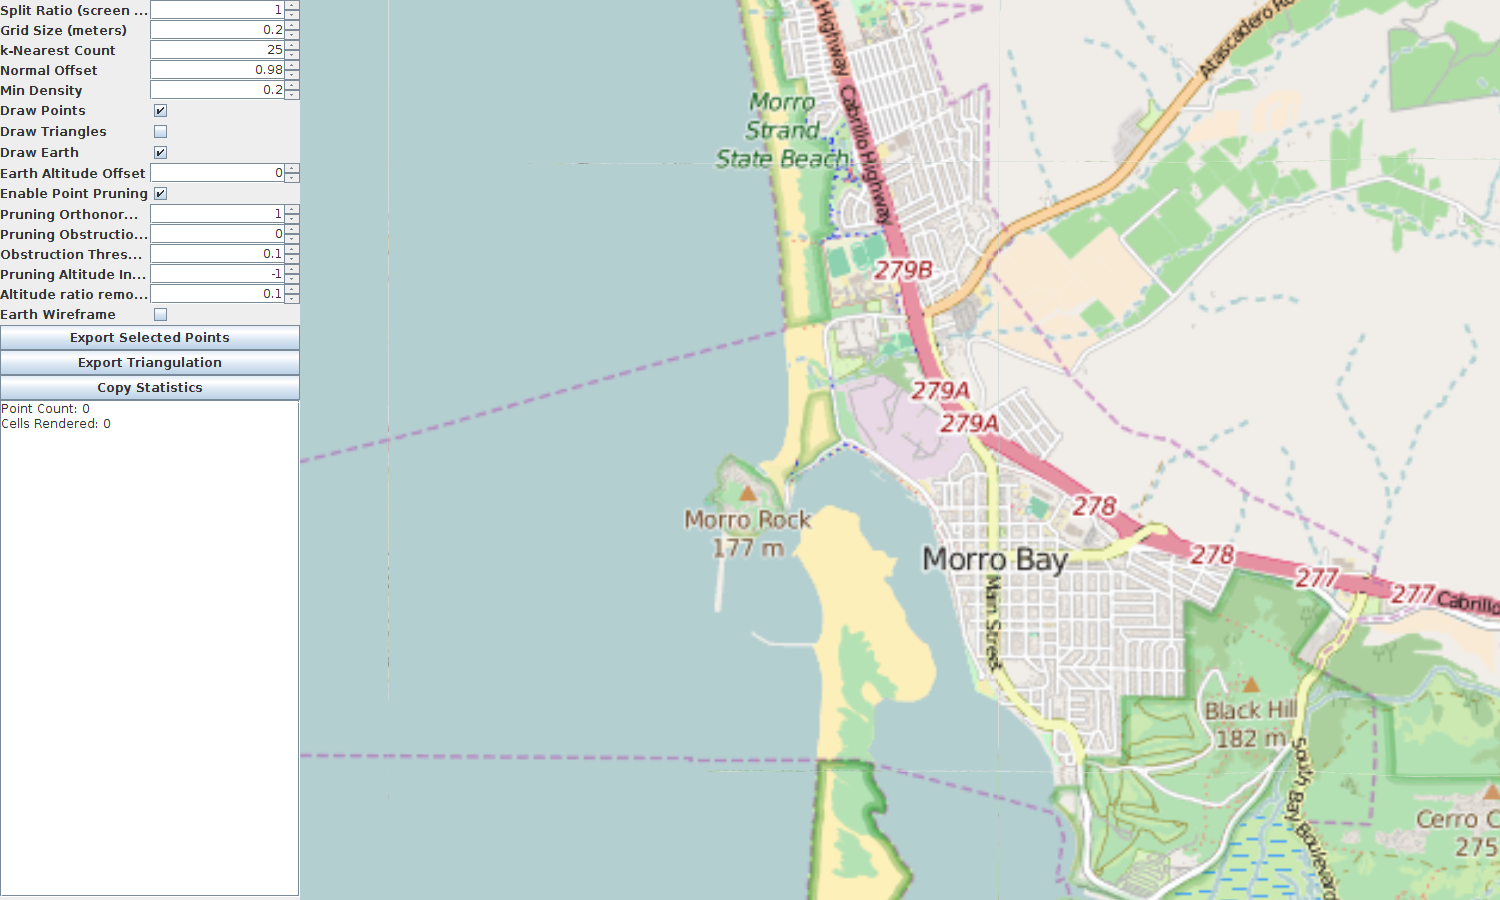
\includegraphics[width=.75\linewidth]{images/earthTiles.png}
  \caption{OpenStreetMap Tiles}
  \label{fig:earthTiles}
\end{center}
\end{figure}

\section{Rendering Component}

The rendering component initially reads the root node and attributes layout
information from the dataset (locally or over the web). It then uses the
bounding volume of the node to determine if it should be rendered or not and if
its children should be queried. It then uses a screen-space level of detail
algorithm to determine how deep to traverse; this depth will be tunable based on
user preference.

The Octree and Icosatree are both supported by the rendering component as their
data structures are identical aside from the number of children their root nodes
may contain. The class TreeRenderable is given a path (either local or HTTP) to
the root of the tree data and a ConnectionType.  Each frame, it does a frustum
culling pass to determine which tree cells should be included in the rendering
step. Then, for each cell it checks its on-screen area. This area calculation is
used to compare against two different thresholds; the first is if this node
should render any points it may contain (50×50 pixels) and the second is if its
children should be checked (200×200 pixels). The nodes are split into two sets;
those that are complete and those that are pending. The complete nodes have
their point data already retrieved while the pending nodes have been created but
are still waiting for their point data to be accessed by the connection thread.
Next, a small portion of the frame time is given over for uploading data to the
graphics card; this is limited in order to keep the visualization at an
interactive frame rate. The vertex buffer implementation is actually a number of
buffer pools, each of which contain a number of vertex buffer objects and the
pool is able to allocate and delete these objects as needed. The tree structure
contains the maximum number of points necessary for any node in the tree; this
is the starting segment size for the buffer pools. The first pool is defined by
a number of segments (100 by default) which can each hold this maximum number of
points per buffer object (byte size equal to the attribute-stride * max points *
segments per buffer). Then, another pool is made by dividing the segment size by
two and continuing this until the smallest buffer object is sliced into segments
less than 100 points long. This allows a number of different sized cells to be
inserted into a buffer that, at least, fills half of its total capacity but also
allows the rendering system to intelligently add, remove, and update cells in
the tree without having to pack or rearrange data on the graphics card every
frame. Below, in \ref{fig:visualization}, is a screenshot of Morro Bay in California; this
is a subset of the San Simeon, CA point cloud dataset and, in total, contains
13,725,592 points. At the current zoom distance and level of detail the
rendering component is only required to render around three million points.

\begin{figure}[htp]
\begin{center}
  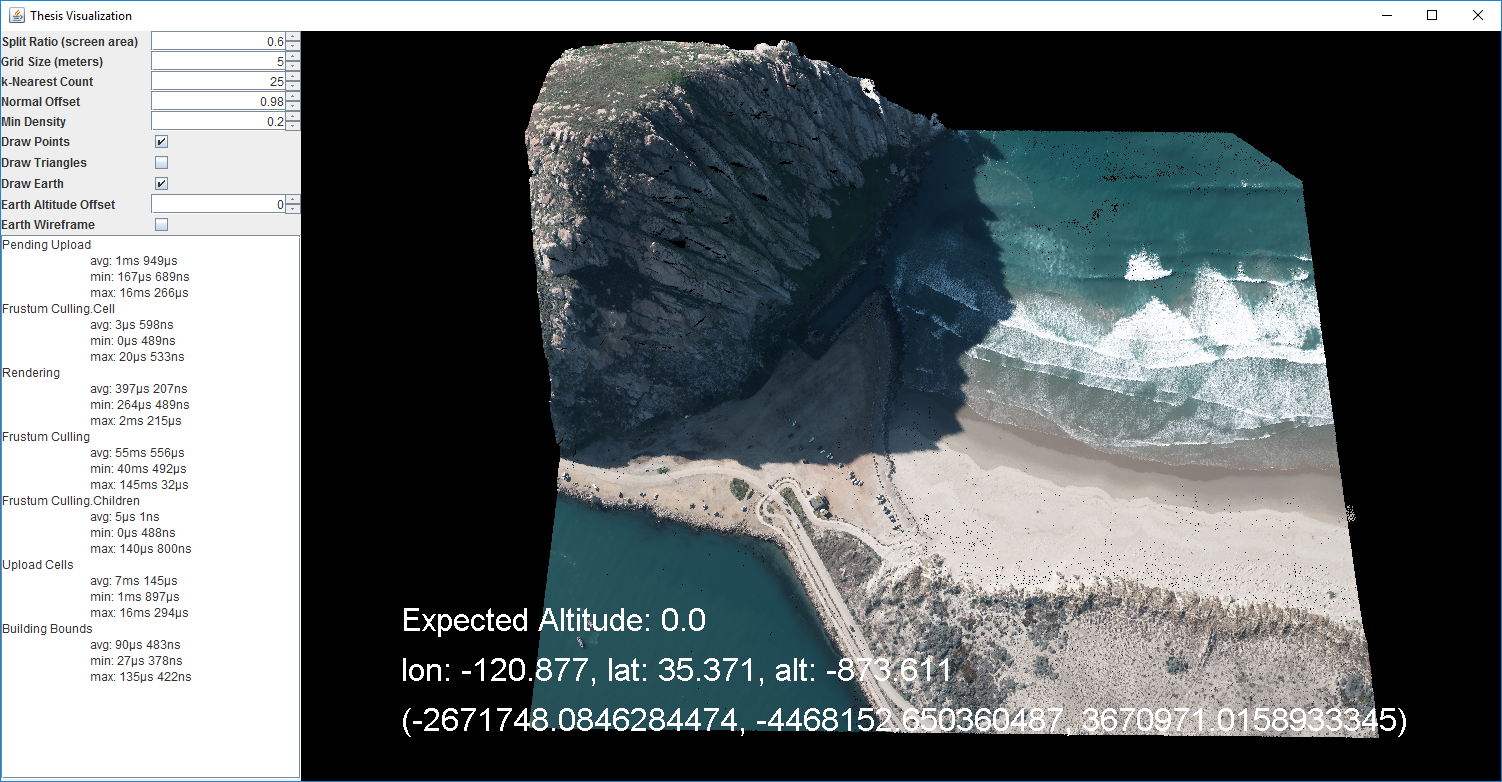
\includegraphics[width=.9\linewidth]{images/visualization.png}
  \caption{Visualization Application with Small Point Cloud}
  \label{fig:visualization}
\end{center}
\end{figure}

The TreeRenderable itself controls how the point data is
displayed in the visualization application. It creates a custom-built vertex
buffer object pool which is then used to store and render the point data. The
buffer pool contains a set of smaller pools internally that are defined by a set
segment size (number of points available in a block) and a number of available
segments. Each of these smaller pools is able to append itself with as many
vertex buffer objects as it needs and uses a global index to find the specific
segment location that is bound to each tree cell. When a segment is cleared, any
empty vertex buffer objects on a segment pool will also be removed in order to
free up memory. When the Tree Cells are uploaded to the GPU, the segment pool
with the smallest segment size that will fit the tree cell's point count will be
selected. Then, the first available index in that cell will be requested and the
tree cell will store this pool index and segment index for rendering later. The
number of internal segment pools is defined by the maximum number of points any
given tree cell will contain in the point cloud collection. \ref{fig:flowchart}
is a flow chart that goes through the steps in the rendering pass for the TreeRenderable.

\begin{figure}[htp]
\begin{center}
  \includegraphics[width=.9\linewidth]{images/TreeRenderer_flowchart.png}
  \caption{TreeRenderer Flow Chart}
  \label{fig:flowchart}
\end{center}
\end{figure}

\section{Selection Algorithm}

The selection algorithm attempts to apply portions of two separate point cloud
selection algorithms to the same set of data. The Screen-Space Operator
Algorithm \cite{1_VAST:VAST11:105-112} is used to define surfaces inside the
point cloud; this is useful for visualizing the walls of buildings and such.
However, the algorithm itself doesn't handle selection of objects. The CAST
algorithm \cite{2_yu:hal-01178051} allows selection of more dense portions of a
point cloud via two-dimensional mouse selection but it requires a dense cloud of
points to handle selection. I have attempted to apply the screen-space lasso and
point density techniques from the CAST algorithm and apply the surface creation
and triangulation algorithm to the resulting selection in order to give a user
more utility when analyzing a point cloud dataset.

The first step of the algorithm is for the user to define the search area. This
is done in the visualization by holding the control key and holding the left
mouse button while defining the lasso area. The shape is automatically connected
to the initial selection point as the user outlines the lasso shape but the
final polygon will be automatically closed the first time the lasso crosses
itself in order to create a closed loop.

Then, a simple volume frustum is created from the camera into the scene along
the screen-space lasso polygon. The tree is searched and any points that are
contained within the lasso are returned. Next, for each point, the k-nearest
neighboring points are queried and a covariance matrix is computed. If the
normal of the best-fit plane of the entire selection is parallel (or within a
user-defined threshold) the point is dropped from the selection. Finally, any
points whose most distant neighbor is further than twice the user-defined grid
size is also removed. This removes any points that are parallel to the ground as
well as any points that are in small groups and aren't useful (less than the
k-nearest limit).

In order to handle triangulation, the Screen-Space Operator Algorithm is used to
determine which points in the selection are unobstructed. This is done by
projecting a ray from each point towards the camera and, if any other point is
within a specified angular distance and closer to the camera than the tested
point, it is removed. These points are then converted into a two-dimensional
plane and a Delaunay triangulation algorithm is used to triangulate them. A map
of the 2D projected point to the original 3D point is used to convert this
triangulation back into a useful triangle mesh. The lasso (\ref{fig:lasso}),
point selection (\ref{fig:pointSelection}), and triangle mesh
(\ref{fig:triangulation}) can be seen below. The follwing is pseudocode for the
Selection Algorithm:

\begin{enumerate}
  \item User Selects Area Of Screen
  \item Create closed polygon from set of screen coordinates
  \item Create projected 3D volume from 2D polygon
  \item Get volume intersection on visible point data
  \item If Pruning enabled, prune points based on user settings
  \begin{enumerate}
    \item Apply the following in User Order
    \begin{itemize}
      \item Orthonormal Pruning
      \begin{enumerate}
        \item Compute global eigenvector for plane normal vector
        \item For-each point, compute engenvector using k-nearest neighbors
        \item if point eigenvector is within user-defined angle of global normal, discard
      \end{enumerate}
      \item Obstruction Pruning
      \begin{enumerate}
        \item For-each point, if any other point is closer to the camera and the angle between the two points is within a user-defined threshold, discard
      \end{enumerate}
      \item Altitude Pruning
      \begin{enumerate}
        \item Compute min/max altitude of all input points
        \item For-each point, if altitude is within user-defined threshold of min value, discard
      \end{enumerate}
    \end{itemize}
  \end{enumerate}
  \item If user enabled, Draw Points
  \item If user enabled, Compute Triangle Mesh
    \begin{enumerate}
      \item Project points to Screen Space
      \item Remove any occluded points
      \item Compute Mesh using Delaunay Triangulation
      \item Project triangulation to World Space
      \item Render Triangle Mesh
    \end{enumerate}
\end{enumerate}

\begin{figure}[htp]
\begin{center}
  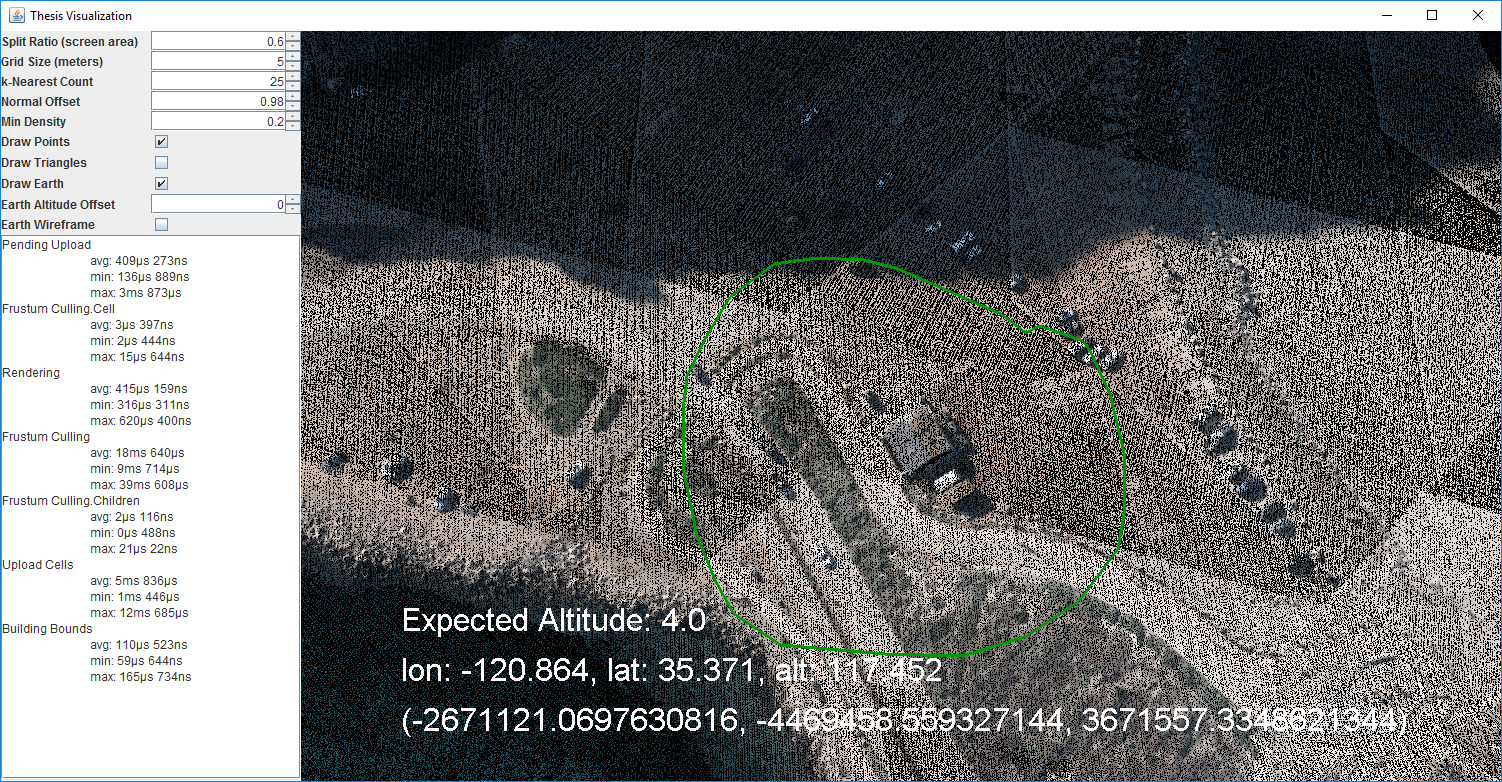
\includegraphics[width=.75\linewidth]{images/lasso.png}
  \caption{Selection Lasso}
  \label{fig:lasso}
\end{center}
\end{figure}

\begin{figure}[htp]
\begin{center}
  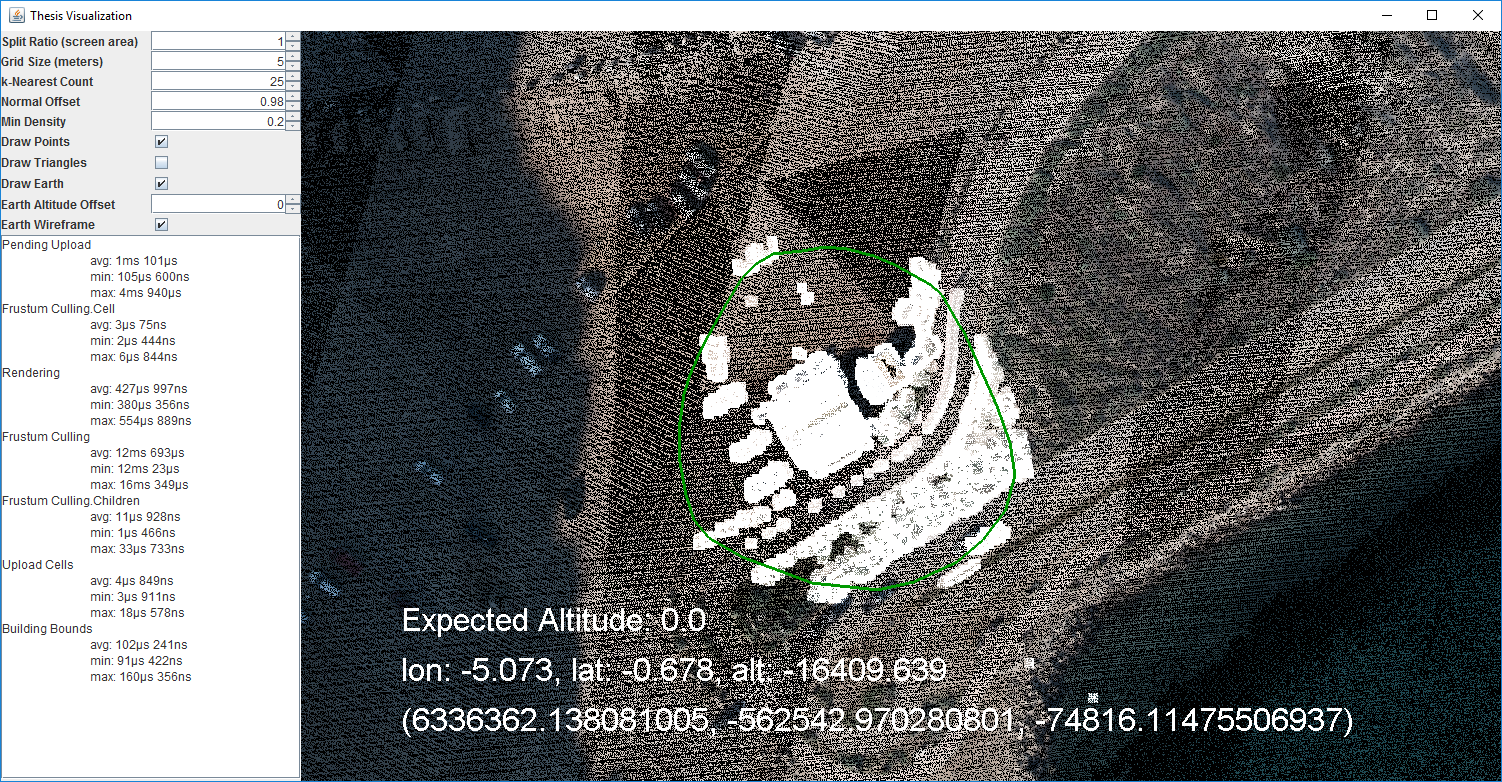
\includegraphics[width=.75\linewidth]{images/pointSelection.png}
  \caption{Point Selection}
  \label{fig:pointSelection}
\end{center}
\end{figure}

\begin{figure}[htp]
\begin{center}
  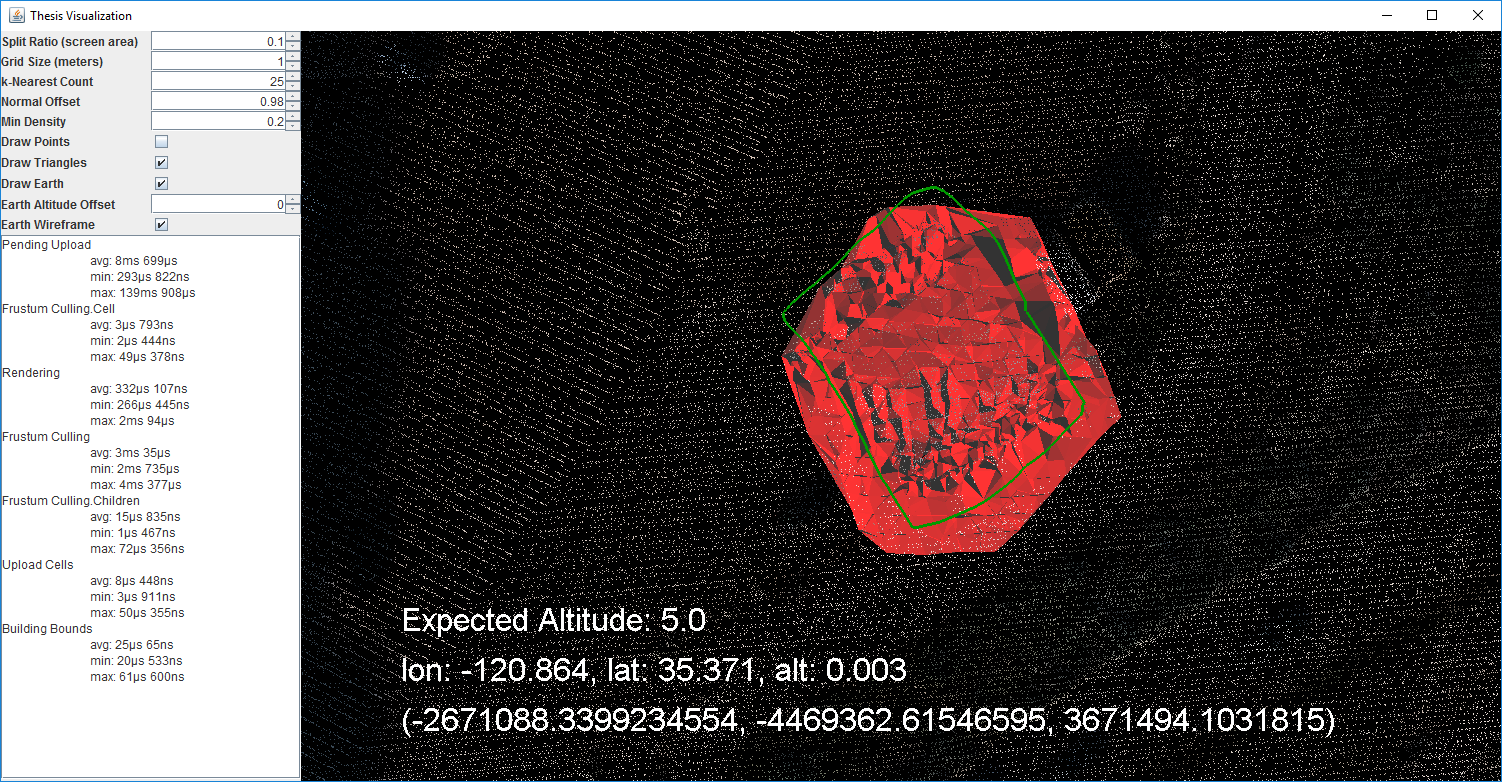
\includegraphics[width=.75\linewidth]{images/triangulation.png}
  \caption{Point Triangulation}
  \label{fig:triangulation}
\end{center}
\end{figure}

\chapter{Analysis}

%% Obviously you need to delete these lines when you have written up your text

\begin{itemize}
\item{}  How did you analyze your hyptothesis? Experiments, what did you think were worth measuring, etc.
\item{}  Based on your measurements and qualititative analyses, how well did your approach work out?
\item{}  Use graphs, tables, and other diagrams to illustrate your analyses.
\item{}  Based on your analyses, how well does your implementation or approach match your hypothesis?
\item{}  What do you deduce from this effort? How would you change or tweak your hypothesis? 

\end{itemize}
\chapter{Conclusions}

\section{Current Status}

The algorithms and data structures are in place and are able to build and
visualize point cloud datasets from raw point data. The data requires values for
X, Y, Z, Red, Green, Blue, Altitude, and Intensity. There is support for custom
sets of attributes for the input point data but it has not been implemented at
this time.

The visualization supports a camera navigation control based on an anchor
location on the Earth's surface as well as a spherical coordinate offset from
the defined anchor. This allows the user to set the point along the surface that
the camera is bound to but gives them the freedom to rotate around it and move
closer to or further from it.

The Earth rendering component supports level of detail so the geometry will
progressively become more or less detailed as the distance from it changes.
Digital Elevation Model data is used to define the altitude about the ellipsoid
for each vertex and Slippy map tiles are supported for imagery (such as
OpenStreetMap or Stamen).

The point selection and triangulation algorithms have been implemented such that
the user can define a number of toggles and thresholds from the visualization
user interface. Then, the user can select a portion of the screen where a lasso
will draw on screen and select any points within its bounds. Next, any pruning
functions will be applied and any triangulation steps will be executed.

The visualization also supports exporting the selected points or resulting
triangulation in the PLY model format.

The performance of the Icosatree was overall promising. The surface-aligned
nature of the tree cells was much more visually pleasing as data was updated in
the visualization and the tree cells were filled more efficiently for better
use of hardware resources. However, sub-optimal tree partitioning values limited
the performance of the system overall as the initialization parameters for the
Tree data structure are much more important to the functionality of the
visualization system with the Icosatree than they are with the Octree. Also, the
triangular prism bounding volume requires more calculations than the
axis-aligned bounding volume and the sub-optimal tree parameters requires more
tree cells to be rendered for the Icosatree so the added complexity was not
offset by limiting the number of required tree cells.

\section{Future Work}

The visualization and data creation software currently supports a very specific
set of input data in order to build the tree data structures and the
visualization assumes specific point attributes will be available (as stated in
the previous section). However, support to allow the user to define what
attributes are applied to the visualization and support for other coordinate
systems, such as longitude, latitude, and altitude instead of XYZ would be
helpful. Also, reading a set of LAS/LAZ files directly would be convenient.

The initial testing of the Icosatree data structure turned out promising.
However, when building the initial Icosatree dataset and deciding what cell
split values to use there were a few glaring issues.

First, more time needs to be taken in selecting proper sub-cell split values for
the Icosatree. Selecting the same values as used with the Octree creation does
not yield comparable results. The Octree cell split values determines an exact
X-Y-Z cell index such that multiplying the split values together give the total
number of cells. Another issue here is that the Octree cells are 90\% unused in
the majority of instances so creating a more dense sub-cell structure is less
likely to cause issues with memory management in the long run; this is not the
case with the Icosatree. The Icosatree cell split values are used to determine
two separate split coordinates; the first is based on the triangular cell face
and the second is based on the depth of the volume. Therefore, the split value
for the Icosatree's depth is only loosely based on the same data as the
Octree; the Octree is axis-aligned so there is no depth in the same way there
is with the Icosatree which is pseudo-surface-aligned (the center points of the
faces are aligned with the surface directly below them but the further from the
center the less aligned they become). The depth split for each still separates
the sub-cells in a similar way; the distance along the axis of separation
creates the same number of new sub-cells. For the top face split value, however,
is used as an index along its edges. The surface of this face is also much less
area than the Octree cells. An Octet and Icosatet of comparable size with split
values of six for each dimension will both turn into 216 sub-cells but the Octet
will take up more than twice the volume so the Icosatet will store many more
point instances in a much smaller volume, not to mention the higher sub-cell
utilization from being more surface-aligned than the Octet.

Second, the dataset creation tool needs to be streamlined, multi-threaded, and
updated to run on a cached file storage system. Storing the working copy of the
tree building data in memory is infeasible for even a moderately-sized dataset.
When testing, the initial dataset was a few gigabytes which fit in memory
without much issue. However, once a larger dataset was selected, an order of
magnitude larger than the original dataset, the in-memory limitations of the
original dataset creation tool were very apparent. The tool was then updated to
use a memory-mapped database for storing the point data (MapDB) but even that
has its limitations. It was not able to create a mapped database for all the
Tree cells being created (could not keep all files mapped at once) so a single
mapped database was used for all the points. This causes some synchronization
slowdowns the larger the dataset becomes. Adding support for in-place file
caching and multi-threading could greatly increase performance of the dataset
creation tool. Unfortunately, the projected completion time for the larger
dataset with the current iteration of the dataset creation tool precluded the
testing of the visualization with a larger point cloud.

Next, the point selection and triangulation portion of the paper could be
optimized further, adding a more real-time option to the visualization. As the
various pieces of the algorithms were developed they were added ad-hoc to the
visualization system. This allowed the pieces to be tested in a modular fashion,
however, it is very likely that much of the calculations done could be
consolidated or simplified. Also, moving many of these calculations off to a
general purpose processing engine such as OpenCL or CUDA, much of the time taken
to calculate output could be sped up considerably.

Last, the visualization tool was not the focus of the work for this paper but
was necessary in order to display and test the results. However, it is a bit
rough around the edges and needs some work. Fixing the graphics pipeline issues
in the current graphics engine would be preferable but replacing it with an Open
Source alternative might be a viable option depending on the time required to
port the current code base to the new platform.

The visualization itself was built on top of a rendering library written by the
author but not intended to support direct manipulation of the camera. For this
paper it was updated to support mouse interaction and a navigation class was
written for intuitive and easy to use controls for moving around an elliptical
surface; in this case, a WGS84 projected Earth. However, the interaction with
these two systems is not perfect and needs some fine tuning, debugging, and
various improvements. Such improvements include support for camera movement
based on velocity and acceleration, frustum to bounding volume intersection
validation, and world-screen coordinate conversion validation.

%%%%%%%%%%%%%%%%%%%%%%%%%%%%%%%%%%%%%%%%%%%%%%%%%%%%%%%%%%%%%%%%%%%%%%%%%%%%%%%

%%%%%%%%%%%%%%%%%%%%%%%%%%%%%%%%%%%%%%%%%%%%%%%%%%%%%%%%%%%%%%%%%%%%%%%%%%%%%%%
\bibliographystyle{plain}
% Single space the bibliography to save space.
\begin{singlespace}
\bibliography{CapstoneBib}
\end{singlespace}
%%%%%%%%%%%%%%%%%%%%%%%%%%%%%%%%%%%%%%%%%%%%%%%%%%%%%%%%%%%%%%%%%%%%%%%%%%%%%%%

%%%%%%%%%%%%%%%%%%%%%%%%%%%%%%%%%%%%%%%%%%%%%%%%%%%%%%%%%%%%%%%%%%%%%%%%%%%%%%%
% The appendices are (of course) optional.
\appendix
\chapter{UML Diagrams}

This is an optional appendix and can be eliminated if you don't have anything 
to share here.


%\chapter{Code Listing}

This is an optional appendix and can be eliminated if you don't have anything 
to share here.


%\chapter{User Manual}

This is an optional appendix and can be eliminated if you don't have anything 
to share here.


% ...
%%%%%%%%%%%%%%%%%%%%%%%%%%%%%%%%%%%%%%%%%%%%%%%%%%%%%%%%%%%%%%%%%%%%%%%%%%%%%%%
\end{document}
